\section{Normalizing Flows}
% Goal: a latent variable model with tractable likelihoods.
\textbf{Idea} \( p_{X;\theta}(x)=p_{Z}(f_{\theta}^{-1}(x))|\text{det}\partial_{x} f_{\theta}^{-1}(x)|\).
\textbf{Require} (1) NN differentiable, invertible, preserve the dim, (2) Jacobian computed efficiently.
\textbf{Trick} triangular matrix to reduce the complexity of Det to \(O(d)\).

Flow Trans:\({x} = f_{k} \circ f_{k-1} \circ \cdots f_{2} \circ f_{1}(z)\), \(p_{x}(x)=p_{z}(f^{-1}(x)) \prod_{k}|\text{det}\partial_{x} f_{k}^{-1}(x)| \)

\textbf{ML} \(\log p_{x}({\mathcal{D}})=\sum_{x \in \mathcal{D}}\ln p_{z}(f^{-1}({x}))+\sum_{k} \ln|\text{det}\partial_{x} f_{k}^{-1}(x)| \).
\textbf{Planner}: \(f(z)={z}+{u h}({w}^{T} {z}+{b})\), \(|\operatorname{det} \partial_{{z}} f |=|1+h^{\prime} {u}^{T} {w}|\).
\textbf{Radial}: \(f({z})={z}+\beta h(\alpha, r)({z}-{z}_{0})\), \(r=|{z}-{z}_{0}|\), \(h(\alpha, r)=(\alpha+r)^{-1}\), \(|\operatorname{det} \partial_{{z}} f| = [1+\beta h(\alpha, r)]^{d-1}[1+\beta h(\alpha, r)+\beta h^{\prime}(\alpha, r) r]\)

\subsection*{Coupling Layer}
\textsf{F}
\(\left(\begin{array}{c}
        y^{A} \\
        y^{B}
    \end{array}\right)=\left(\begin{array}{c}
        h(x^{A}, \beta(x^{B})) \\
        x^{B}
    \end{array}\right),\)
\textsf{R} \(\left(\begin{array}{l}
        x^{A} \\
        x^{B}
    \end{array}\right)=\left(\begin{array}{c}
        h^{-1}(y^{A}, \beta(y^{B}))) \\
        y^{B}
    \end{array}\right),\)
Jacob \(\left(\begin{array}{cc}
        h^{\prime} & h^{\prime} \beta^{\prime} \\
        0          & 1
    \end{array}\right).\)\\
\(h(x) = (h(x_{1}), \ldots, h(x_{n}))^{\top}\) element-wise. \( \partial_{x^{\top}} h=\operatorname{diag}(h^{\prime}(x_{1}), \ldots, h^{\prime}(x_{n}))\).

Continuous NF: model infinite number of trans with proper temporal discretization. Neural ODE.

\begin{center}
    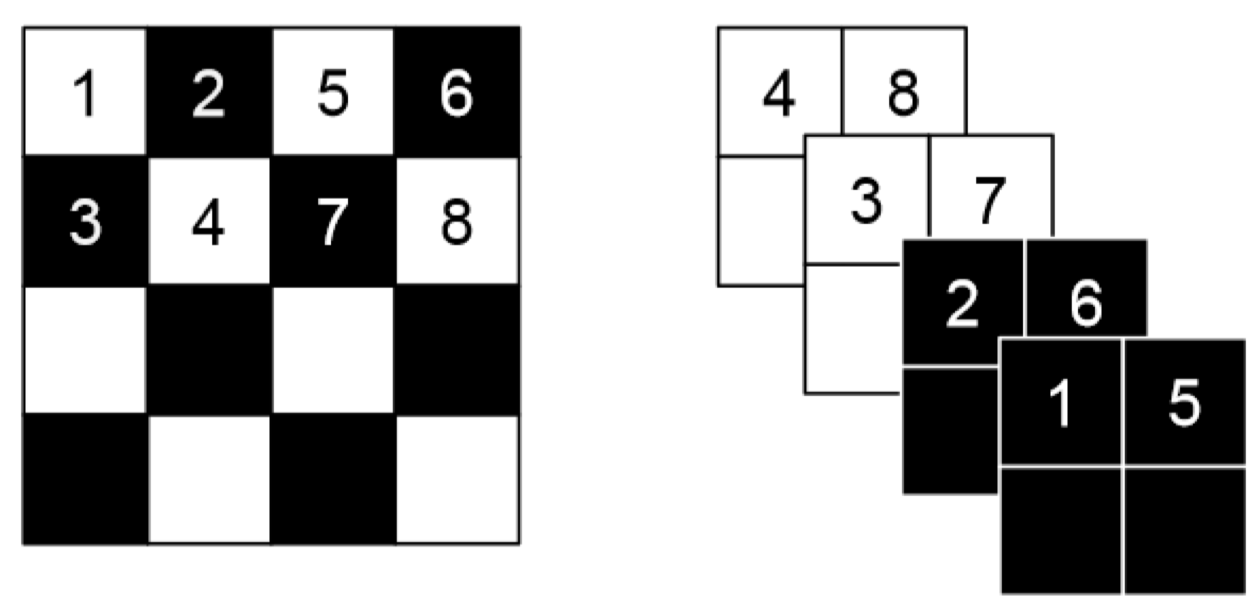
\includegraphics[width=0.8\columnwidth]{figures/coupling_layer.png}
\end{center}

\subsection*{NF in CV, Flow Block (FB)}

In NF, part of output processed, else passed to latter layer. Shuffle needed and different among papers.

Squeeze \& split: reduce spacial dimension and distribute them into the channel, splitting in channel. \((i,j)\): spacial idx.

\subsection*{FB1 - activation norm}
Scale and bias per channel, sim to BN, data depend, trainable.
\textsf{F} \( y_{i, j}={s} \odot x_{i, j}+{b}\),
\textsf{R} \( {x}_{i, j}=({y}_{i, j}-{b}) / {s}\),
\textsf{LogDet} \(\mathrm{H} \cdot W \cdot \operatorname{sum}(\log |s|)\).

\subsection*{FB2 - invertible 1x1 conv}

\textsf{F} \({y}_{i, j}={W} {x}_{i, j}\)
\textsf{R} \({x}_{i, j}={W}^{-1} {y}_{i, j}\)
\textsf{LogDet} \(h \cdot w \cdot \log |\operatorname{det}{W}|\), \({W}:[c \times c]\),
\(O(c^3)\) for \(|\operatorname{det}{W}|\)  reduce to \(O(c)\) by \({W}={P L}({U}+\operatorname{diag}({s}))\), \(\log |\operatorname{det}{W}|=\operatorname{sum}(\log |{s}|)\).


\subsection*{Fb3 - (conditional) coupling layer}

\textsf{F} \({x}_{a}, {x}_{b}=\operatorname{split}({x})\), \((\log {s}, {t})=\mathrm{NN}({x}_{b}) \), \({s}=\exp (\log {s})\), \( {y}_{a}={s} \odot {x}_{a}+{t}\), \({y}_{b}={x}_{b}\), \({y}=\operatorname{concat}({y}_{a}, {y}_{b})\),
\textsf{R} \({y}_{a}, {y}_{b}=\operatorname{split}({y})\), \((\log {s}, {t})=\mathrm{NN}({y}_{b})\), \({s}=\exp (\log {s})\), \({x}_{a}=({y}_{a}-{t}) / {s}\), \({x}_{b}={y}_{b}\), \({x}=\operatorname{concat}({x}_{a}, {x}_{b})\),
\textsf{LogDet} \(\operatorname{sum}(\log (|{s}|))\).
\textbf{Conditional operation} \(\beta(x^{B};C)\).

\begin{center}
    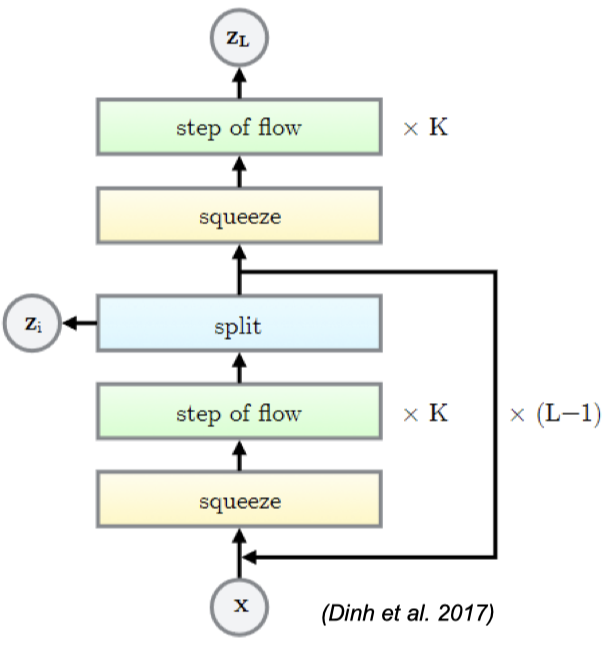
\includegraphics[width=0.5\columnwidth]{figures/flow_block.png}
\end{center}

\subsection*{Application}

\textbf{Super-Res Flow} learns a distribution of HR variants. Cond on a low-res image.  Pretrained CNN encodes a low-resolution image: \({u}=g_{\theta}({x})\) inject to actnorm, affects all channels and spatial locations. \textsf{F} \({h}^{n+1}=\exp (f_{{\theta}, s}^{n}({u})) \cdot {h}^{n}+f_{{\theta}, b}({u})\), \textsf{R} \({h}^{n}=\exp (-f^{n} {\theta}, s({u})) \cdot({h}^{n+1}-f^{n} {\theta}, b({u}))\), \textsf{LogDet} \(\sum_{i j k} f^{n} {\theta}_{, s}({u})_{i j k}\).


\textbf{StyleFlow}(cmp to StyleGAN) Replace mapping network with a continuous normalizing flow, Condition on image attributes.


\textbf{C-Flow} 

Conditioning \(Flow_A\): Standard affine coupling layer, to images.

Conditioned \(Flow_B\): trans param conditioned on, to point cloud, sketch, seg, etc.

\textbf{Enable} (1) (multimodal) image-to-image mapping (2) style transfer (3) image manipulation (4) 3D point cloud reconstruction from images.

\textbf{APP} Probabilistic Modeling for Human Mesh Recovery

\subsection*{Difficalty for geneartive model}
Evaluating \(\log p(x)\) is hard and usually computationally not tractable.
